\documentclass[12pt,a4paper]{article}

\usepackage[a4paper,margin=1in]{geometry}
\usepackage[T1]{fontenc}
\usepackage{lmodern}
\usepackage{microtype}
\usepackage{booktabs}
\usepackage{longtable}
\usepackage{array}
\usepackage{enumitem}
\usepackage{xcolor}
\usepackage{hyperref}
\usepackage{tikz}
\usetikzlibrary{arrows.meta,positioning,shapes.geometric}
\usepackage{listings}
\usepackage{fancyhdr}

\hypersetup{colorlinks=true,linkcolor=blue!60!black,urlcolor=blue!60!black}
\pagestyle{fancy}
\fancyhf{}
\lhead{DataSim}
\rhead{Project Proposal and Database Design}
\cfoot{\thepage}
\setlist{nosep,leftmargin=*}
\setlength{\parindent}{0pt}
\setlength{\parskip}{6pt}

\lstset{basicstyle=\ttfamily\small,breaklines=true,frame=single,columns=fullflexible}
\newcommand{\datasim}{\textbf{DataSim}}

\title{\textbf{DataSim: A Friendly Simulation Lab for Relational Database Systems}}
\author{Akshat Raj \and Vishal Vivek \and Mohit Kumar}
\date{26 September 2026}

\begin{document}
\maketitle

\begin{center}
\textbf{Course:} Database Management Systems\\
\textbf{Repository:} \url{https://github.com/albertaj23/DataSim}
\end{center}

\section*{Contributors}
\begin{center}
\begin{tabular}{ll}
\toprule
\textbf{Reg. No.} & \textbf{Name}\\
\midrule
24BCE0043 & Akshat Raj\\
24BCE2877 & Vishal Vivek\\
24BCE2878 & Mohit Kumar\\
\bottomrule
\end{tabular}
\end{center}

\tableofcontents
\newpage

\section{Project Title}

\textbf{DataSim: A Friendly Simulation Lab for Relational Database Systems.}

\textbf{Music scenario:} Coordinating shared listener accounts and concurrent playback across multiple devices.

\section{Introduction and Background}

Database systems support applications where many users and devices read and modify shared data at the same time. A database may appear correct during a single-user demonstration but behave incorrectly when concurrent requests arrive together. Examples include lost updates, inconsistent reads, race conditions, lock waits, deadlocks, and constraint violations.

\datasim{} is an interactive database simulation lab that makes these behaviors visible. It provides friendly user interfaces for running repeatable scenarios and technical views for examining transactions, locks, constraints, isolation levels, and results. Music playback is used as an understandable example: one listener account may be active on several devices, but a stream limit must remain correct even when many devices press Play simultaneously.

The music domain is an example rather than a limitation. The same simulation approach can be extended to reservations, inventory, ticketing, banking, collaborative editing, or any system with shared state and concurrent users.

\section{Problem Statement}

In a multi-device music service, several devices belonging to one listener account may attempt to start playback at nearly the same time. Each request can read the same database state before writing a new playback session. If the operations are not coordinated correctly, more sessions may become active than the account's permitted limit.

The project addresses the following problem:

\begin{quote}
How can a relational DBMS maintain a correct, real-time shared state under concurrent operations, and what correctness and performance trade-offs are introduced by different transaction, isolation, locking, and constraint strategies?
\end{quote}

\datasim{} also demonstrates the lost-update problem. When many listeners finish the same song concurrently, independent read-modify-write operations may overwrite one another and produce an incorrect play count.

\section{Objectives}

\begin{enumerate}
\item Model users, devices, songs, playback sessions, events, and experiment results in a normalized relational database.
\item Demonstrate concurrency anomalies using reproducible scenarios rather than only theoretical examples.
\item Compare naive operations, transactions, serializable isolation, pessimistic locking, optimistic version checks, unique constraints, triggers, and a Redis lease strategy.
\item Show how isolation levels affect visibility, blocking, deadlocks, and correctness.
\item Visualize transaction schedules, lock information, wait-for relationships, rollbacks, and invariant checks.
\item Simulate a scalable crowd of virtual music listeners using real database transactions.
\item Provide a friendly interface for learners and a technical interface for detailed inspection.
\item Persist experiment configurations and results so that runs can be compared and analyzed.
\item Keep the platform extensible so future scenarios can reuse the same simulation and measurement patterns.
\end{enumerate}

\section{Scope of the Project}

\subsection{Included}
\begin{itemize}
\item MySQL 8.4 relational database using the InnoDB storage engine.
\item Schema for accounts, devices, songs, playback sessions, playback events, and experiment runs.
\item Account-level playback limits and lease-based session expiry.
\item Multiple concurrency-control strategies for the same business operation.
\item Lost-update experiments using a shared song play counter.
\item Transaction Stepper for statement-by-statement execution of two transactions.
\item Concurrency Lab for repeated race experiments and measurement.
\item Simulation Control Room for virtual listeners and real database traffic.
\item InnoDB lock and wait-for information where available.
\item Invariant checks for stream limits, leases, duplicate sessions, and audit consistency.
\item React web interface, Node.js/TypeScript API, Docker setup, and automated tests.
\end{itemize}

\subsection{Excluded}
\begin{itemize}
\item Real audio streaming, media storage, or content licensing.
\item Production authentication, authorization, subscriptions, or payment processing.
\item Production-scale cloud deployment or guaranteed multi-region availability.
\item Personalization, recommendations, advertising, and social networking.
\item Any claim that the implementation represents the internal design of a commercial streaming service.
\item Unlimited arbitrary workloads; the simulator uses bounded, controlled scenarios for repeatability.
\end{itemize}

\section{Requirement Analysis}

\subsection{Users}
\begin{longtable}{p{0.25\textwidth}p{0.65\textwidth}}
\toprule
\textbf{User} & \textbf{Main needs}\\
\midrule
Student or learner & Understand DBMS concepts through guided visual scenarios.\\
Demonstrator or instructor & Run repeatable experiments and explain anomalies.\\
Technical user & Inspect SQL effects, locks, transactions, constraints, and results.\\
Developer & Add new database strategies or scenarios without replacing the platform.\\
\bottomrule
\end{longtable}

\subsection{Data to be stored}
\begin{itemize}
\item \textbf{Account:} username, stream limit, conflict policy, state version, and laboratory flag.
\item \textbf{Device:} account ownership, device name/type, and last-seen time.
\item \textbf{Song:} title, artist, and play counter used by the lost-update experiment.
\item \textbf{Playback session:} device, account, song, status, position, timestamps, lease, and strategy.
\item \textbf{Playback event:} state transition, references, timestamp, version, request id, and details.
\item \textbf{Experiment run:} type, strategy, configuration, outcomes, latency, throughput, violations, and batch id.
\end{itemize}

\subsection{Required operations}
\begin{enumerate}
\item Look up an account and its devices.
\item Start, pause, resume, release, or stop playback.
\item Renew a playback lease through a heartbeat.
\item Take over playback according to a conflict policy.
\item Reject expired, preempted, or stale device requests.
\item Switch the active concurrency strategy.
\item Run stream-limit and lost-update experiments.
\item Step through two transactions one statement at a time.
\item Start, pause, resume, repair, and stop a crowd simulation.
\item Inspect live state, audit events, locks, and experiment history.
\end{enumerate}

\subsection{Information to retrieve and analyze}

The system retrieves active sessions per account, invariant status, lost updates, transaction outcomes, retries, deadlocks, rollbacks, lock waits, latency percentiles, throughput, violation counts, event timelines, and strategy comparisons.

\subsection{Functional requirements}
\begin{enumerate}
\item The system shall store account, device, song, session, event, and experiment data.
\item The system shall support concurrent playback claims from multiple devices.
\item The system shall implement and compare multiple protection strategies.
\item The system shall record experiment configurations and results.
\item The system shall expose invariant and consistency checks.
\item The system shall provide friendly scenario controls and technical inspection views.
\item The system shall reject expired, preempted, or stale device operations.
\end{enumerate}

\subsection{Non-functional requirements}

The system must provide correctness, repeatability, observability, bounded scalability, maintainability, local portability, and usability. Experiments must be controlled and their results must be persisted for later comparison.

\section{Database Selection and Justification}

\subsection{Selected technology}
\begin{itemize}
\item \textbf{Database:} MySQL 8.4.
\item \textbf{Type:} Relational database management system.
\item \textbf{Storage engine:} InnoDB.
\item \textbf{Additional component:} Redis 7 for an optional lease-based comparison strategy.
\item \textbf{Application stack:} Node.js, TypeScript, Express, React, and Socket.IO.
\end{itemize}

A relational DBMS is appropriate because \datasim{} studies transactions, isolation levels, row and gap locks, constraints, foreign keys, deadlocks, and consistency of related entities. MySQL/InnoDB provides these mechanisms in a real database engine, allowing the project to measure actual behavior rather than simulate every rule in application code.

MySQL was selected because InnoDB supports ACID transactions and multiple isolation levels; row-level and next-key locking; foreign keys, unique constraints, checks, triggers, and generated columns; performance-schema lock inspection; and reproducible Docker-based execution. Redis is included as a separate comparison point to show how an external key-value lease gate can coordinate access while MySQL remains the durable relational source of truth.

\section{Data Model / Database Design}

\subsection{Main entities and attributes}
\begin{longtable}{p{0.22\textwidth}p{0.46\textwidth}p{0.22\textwidth}}
\toprule
\textbf{Entity} & \textbf{Important attributes} & \textbf{Keys/constraints}\\
\midrule
\texttt{account} & id, username, max streams, conflict policy, state version, lab flag & PK, unique username, checks\\
\texttt{device} & id, account, name, type, last seen & PK, FK, unique account/name\\
\texttt{song} & id, title, artist, play count & PK, non-negative count\\
\texttt{playback\_session} & device, account, song, status, position, lease, strategy & PK, composite FK, song FK, indexes\\
\texttt{playback\_event} & state transition, references, version, request id, details & PK, unique request id\\
\texttt{experiment\_run} & type, strategy, config, outcomes, latency, throughput & PK, batch indexes\\
\bottomrule
\end{longtable}

\subsection{Entity-relationship diagram}

\begin{center}
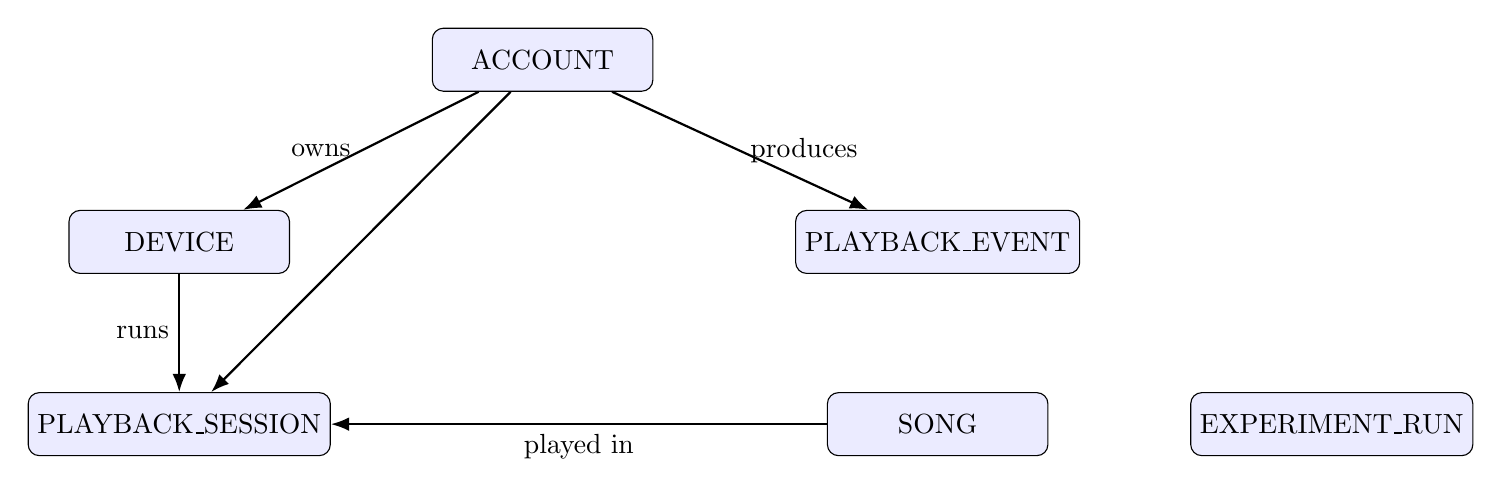
\begin{tikzpicture}[node distance=1.5cm and 1.8cm, entity/.style={draw,rounded corners,fill=blue!8,minimum width=2.8cm,minimum height=0.8cm,align=center}, rel/.style={-{Latex},thick}]
\node[entity] (account) {ACCOUNT};
\node[entity,below left=of account] (device) {DEVICE};
\node[entity,below right=of account] (event) {PLAYBACK\_EVENT};
\node[entity,below=of device] (session) {PLAYBACK\_SESSION};
\node[entity,below=of event] (song) {SONG};
\node[entity,right=of song] (run) {EXPERIMENT\_RUN};
\draw[rel] (account) -- node[left]{owns} (device);
\draw[rel] (account) -- node[right]{produces} (event);
\draw[rel] (device) -- node[left]{runs} (session);
\draw[rel] (account) -- (session);
\draw[rel] (song) -- node[below]{played in} (session);
\end{tikzpicture}
\end{center}

\subsection{Relational schema}

\begin{lstlisting}
ACCOUNT(account_id PK, username UNIQUE, max_streams, conflict_policy,
        state_version, is_lab)

DEVICE(device_id PK, account_id FK -> ACCOUNT, device_name,
       device_type, last_seen_at, UNIQUE(account_id, device_name))

SONG(song_id PK, title, artist, play_count)

PLAYBACK_SESSION(session_id PK, device_id, account_id, song_id FK -> SONG,
                 status, position_ms, started_at, lease_expires_at,
                 ended_at, strategy,
                 FK(device_id, account_id) -> DEVICE(device_id, account_id))

PLAYBACK_EVENT(event_id PK, account_id, device_id, session_id, event_type,
               state_version, client_request_id, created_at, detail,
               UNIQUE(device_id, client_request_id))

EXPERIMENT_RUN(run_id PK, experiment, strategy, config, outcomes,
               violations, p50_ms, p95_ms, throughput, batch_id, created_at)
\end{lstlisting}

\subsection{Keys and constraints}
\begin{itemize}
\item Primary keys identify every account, device, song, session, event, and run.
\item Foreign keys preserve ownership and reference integrity.
\item A composite foreign key ensures that a session's device belongs to its recorded account.
\item Unique username and account/device-name constraints prevent duplicate identities.
\item A unique device/request-id constraint makes state-changing requests idempotent.
\item Status, policy, stream-limit, position, and counter checks reject invalid values.
\item An optional generated-column unique index demonstrates declarative protection for one active session per account.
\item The main stream-limit rule is a predicate over multiple rows, so it requires concurrency control rather than only a primary key.
\end{itemize}

\textbf{Core invariant:} For every account, the number of \texttt{PLAYING} sessions with an unexpired lease must be less than or equal to \texttt{max\_streams}.

\subsection{Normalization}

The core schema follows third normal form. Each table represents one main entity or event type; attributes are atomic; non-key attributes depend on the whole key; and device, song, event, and experiment details are not unnecessarily duplicated. The session table intentionally stores both \texttt{device\_id} and \texttt{account\_id} because account-level queries and locking are central to the workload. The composite foreign key keeps this controlled denormalization consistent.

\section{System Architecture / Workflow Diagram}

\subsection{High-level architecture}

\begin{center}
\begin{tikzpicture}[node distance=1.4cm and 1.2cm, block/.style={draw,rounded corners,fill=green!10,minimum width=2.7cm,minimum height=0.9cm,align=center}, db/.style={draw,cylinder,shape border rotate=90,aspect=0.3,fill=orange!15,minimum width=2.3cm,minimum height=1cm,align=center}, arr/.style={-{Latex},thick}]
\node[block] (users) {Users and\learners};
\node[block,right=of users] (ui) {React web\interface};
\node[block,right=of ui] (api) {Node.js API\and services};
\node[db,right=of api] (mysql) {MySQL 8.4\InnoDB};
\node[db,below=of mysql] (redis) {Redis 7\optional};
\node[block,below=of api] (output) {Checks, metrics,\timelines, verdicts};
\draw[arr] (users) -- (ui);
\draw[arr] (ui) -- (api);
\draw[arr] (api) -- (mysql);
\draw[arr] (api) -- (redis);
\draw[arr] (mysql) -- (output);
\draw[arr] (output) -- (ui);
\end{tikzpicture}
\end{center}

\subsection{Scenario workflow}

\begin{enumerate}
\item A user selects a scenario and concurrency strategy in the React interface.
\item The interface sends a playback, experiment, or simulation request to the Node.js API.
\item The service begins a MySQL transaction and reads the relevant shared state.
\item The selected strategy applies locking, isolation, optimistic checks, constraints, or an external lease.
\item MySQL returns a grant, rejection, wait, deadlock, rollback, or conflict result.
\item The service commits or rolls back, records an event or experiment result, and publishes committed state.
\item The interface displays updated sessions, metrics, checks, timelines, and technical diagnostics.
\end{enumerate}

\subsection{System output}

The system produces friendly playback and simulation views, live listener/device state, strategy verdicts, transaction schedules, lock and wait information, experiment history, latency and throughput measurements, violation counts, and CSV/Markdown results for analysis.

\section*{Conclusion}

\datasim{} combines a practical relational schema with an interactive laboratory for studying database behavior under concurrency. The music playback example makes shared state easy to understand, while the underlying design focuses on general DBMS concepts applicable to many domains. By connecting a friendly interface to real MySQL transactions and measurable outcomes, the project shows how database design choices affect correctness, performance, and scalability.

\end{document}
